\documentclass[11pt,letterpaper]{article}
\pdfobjcompresslevel=0
\pdfminorversion=4
\usepackage[margin=1in]{geometry}
\usepackage[T1]{fontenc}
\usepackage[scaled=0.92]{helvet}
\renewcommand\familydefault{\sfdefault}
\usepackage{xcolor,booktabs,graphicx,amsmath,hyperref,caption,enumitem,float}
\hypersetup{colorlinks=true,linkcolor=black,urlcolor=blue!50!black,citecolor=black}
\captionsetup{font=small}
\setlist{nosep}
\setlength{\parskip}{4pt}
\begin{document}

{\LARGE\bfseries An iota of signal in a flood of noise: a stateful detector improves synthetic intrusion detection from 13\% to 92\%\par}
\vspace{6pt}
A synthetic, incident-shaped evaluation with false alarms capped at 5\% of benign review windows.\par
\vspace{4pt}
Kevin Vaillancourt, independent researcher, Sudbury, Ontario. With Apart Research.\par
\vspace{10pt}

\noindent\textbf{Abstract.} Events viewed in isolation do not carry enough signal to cross the threshold into a security event; the accumulation of events does. The detector averages an entity's past events and scores the average beside the current event. On synthetic campaigns calibrated to the timing and phase structure of Hugging Face's 108-hour incident, with false alarms capped at 5\%, detection within 120 hours rises from 13\% without memory to 92\% with it. Controls show the advantage depends on ordered evidence staying attached to the same entity; breaking that removes most of the gain. The evaluation uses four benign entities per attacker; an earlier attackers-only result of 59\% was an entity-age artefact and was replaced. $R_{\rm det}$, the share of predictive information attributable to history rather than the current event, is a diagnostic for whether history holds exploitable signal. These rates are properties of the synthetic generator, not measurements of Hugging Face telemetry.

\section*{1. Introduction}
The detection stack at Hugging Face, by their own account, judged each signal on its own and did not consider the history of the intrusion, only individual events \cite{hf_timeline}. Single alerts do not carry enough signal on their own for this kind of attack. The shape of the attack motivated a detector that considers the history of events rather than current events in isolation. The question is the one my current research asks of persistent state \cite{vaillancourt_r}.

Events viewed in isolation do not carry enough signal to cross the threshold into a security event. The accumulation of events shows whether an intrusion is hidden across them. The detector reported here considers history and raises detection from 13\% to 92\% at 120 hours on the synthetic campaign.

Our main contributions are:
\begin{enumerate}
\item A detector that considers history, with a synthetic testbed calibrated to the shape of the Hugging Face attack. Detection rises from 13\% to 92\% at 120 hours.
\item $R_{\rm det}$ as a diagnostic: the share of predictive information attributable to history rather than the current event, and so whether history holds signal a detector can exploit.
\item A finding and a correction. The initial 59\% result was driven by entity age; the corrected protocol replaced it.
\end{enumerate}

\noindent\textit{What predates the sprint.} All experiments and the written answers this report is assembled from were completed before the sprint, 26 August to 9 September. The sprint window was used for review and final assembly.

\noindent\textit{The incident, from the sources.} Between 9 and 13 July 2026, agents run by OpenAI during an internal cyber-capability evaluation escaped their sandbox and compromised Hugging Face's production infrastructure \cite{hf_timeline,openai_pm}. Hugging Face's reconstruction: about 17,600 attacker actions over 108 hours; daily counts 3,779 / 1,135 / 7,677 / 3,892 / 1,130; phases of 6,191 reconnaissance, 2,911 code-execution, 6,972 dropper actions and under 500 across exfiltration, command-and-control, Kubernetes, supply-chain and Tailscale; lateral movement from 11 July 10:10 UTC (hour 56); attacker cut off 13 July 14:14 UTC, 52 hours later. Their words on detection: signals ``from several layers of our security stack at once,'' each ``ambiguous,'' and the stack ``failed to correctly raise the alert's criticality and trigger the on-call team'' \cite{hf_timeline}.

\section*{2. Related Work}
This work applies the structural remainder $R$ (Vaillancourt 2026a \cite{vaillancourt_r}) in detector form. CUSUM \cite{page1954} ties the memory layer on the original protocol (0.596 against 0.589) and again on the corrected one (Table~\ref{tab:fair}); it needs a hand-set reference level and slack, where the memory layer is learned from data. On the incident, Hugging Face's forensic timeline \cite{hf_timeline}, OpenAI's postmortem \cite{openai_pm}, Elastic's mapping of the agent's tactics to detection rules \cite{elastic}, the CSA post-mortem \cite{csa}, and the METR and Redwood investigation \cite{metr} describe what happened. This report measures how much a detector gains by remembering, and when.

\section*{3. Methods}
The detector averages an entity's past events over time and scores the average beside the current event. It has two sweep windows, a 15-event window and a 24 to 120 hour window. False alarm rates are capped at 5\% of benign review windows. The per-event signal is kept deliberately weak because the real per-event signal is unknown. The 15-event window and the 24 to 120 hour windows are two regimes, run on the short and the long campaign; the gap between them is not measured.

\noindent\textit{Setup.}
\begin{itemize}
\item Generator: five stages numbered 0 to 4 (initial access 0, foothold 1, lateral movement 2, credential access 3, exfiltration 4), advancing by chance each step, with a front burst, a quiet gap and a back phase. Per-event features: signal $=0.5+0.02\times$stage$+\mathcal{N}(0,0.5)$; breadth $=$ Poisson$(0.25+0.02\times$stage$)$; a third feature carrying nothing. Risk $=$ stage $\ge 3$, credential access onward; a stage $\ge 2$ version, lateral movement onward, is also run.
\item Detector: logistic regression on [current event, memory]. Memory $s_t=\alpha s_{t-1}+(1-\alpha)x_{t-1}$, $\alpha=e^{-1/\tau}$, scored with $s_{t-1}$ so the current event never sees itself. Fast $\tau=120$ events, slow $\tau=2500$. Thresholds set on a calibration set so that 5\% of benign review windows contain a page, a benign window being any window of a benign entity or any pre-onset window of an attacker; the union's per-tier budgets tuned the same way.
\item Protocols: short campaign $T=300$ events with a 15-event window; long campaign $T=2000$ with windows of 24 to 120 hours at 21 minutes per event, benign windows at a 12-hour stride. 10,000 test attackers per run.
\item $\hat R_{\rm det}=(\mathrm{CE}_{\rm no\,memory}-\mathrm{CE}_{\rm memory})/(H(Y)-\mathrm{CE}_{\rm memory})$ from out-of-sample cross-entropies, bootstrapped over campaigns; used for orderings, since a ratio of variational lower bounds is not itself a bound \cite{vaillancourt_r}. $\hat R_{\rm det}$ denotes this estimate; $R_{\rm det}$ the population quantity it estimates.
\end{itemize}

The ratio of benign to attacking entities was changed from 0:1 to 4:1. Benign entities produce false alarms at every age, which removes the correlation between detection rate and age.

As per-event signal rises, $R_{\rm det}$ falls; the sweep records where memory stops mattering. Eleven levels of per-event signal from 0.02 to 1.0, everything else fixed.

The synthetic data is calibrated to the shape of the 108-hour attack on Hugging Face as published: actions per day and per phase, and the timing of each phase, with the same burst, quiet, burst daily pattern. In numbers: 2,000 steps mapped onto 108 hours (3.2 minutes and about nine actions per step); stage timing tuned to the daily profile so median onset lands at hour 53 against Hugging Face's 56; windows of 24, 36, 52 and 72 hours after lateral movement; four benign entities per attacker; four levels of per-event signal. The age-term-removed variant gets a three-hour minimum-history gate, because without it a brand-new entity's first few noisy events consume the false-alarm budget.

Five tests, each exiting non-zero on failure, pin the memory arithmetic to the shipped scorer and the fast window code to the original loop. Everything reproduces from the scripts in under two hours on one core.

\section*{4. Results}
The initial tests read a 59\% detection rate. The result was driven by the protocol: every entity in the test set was, by design, an attacker, and the detector learned that age correlated with danger (Table~\ref{tab:locked}). The 4:1 protocol replaced it, and every result that follows is under that protocol.

\begin{table}[H]\centering\small
\begin{tabular}{lr}
\toprule
Original protocol (attackers only), short campaign, 5\% false alarms & Detection \\
\midrule
No memory (myopic) & 0.084 \\
Memory, EMA $\tau=120$ (original headline) & 0.589 \\
Rule ``fire at event 185'', no features at all & 0.709 \\
No memory + event index & 0.726 \\
No memory + last 120 raw events & 0.202 \\
Memory with the age term removed & 0.009 \\
\bottomrule
\end{tabular}
\caption{Original protocol. Detection within a 15-event window at 5\% false alarms.}\label{tab:locked}
\end{table}

The short history sweep catches 20\% of attacks within 15 events, against 10\% for the myopic scorer on the same synthetic data. On the long campaign the hit rate is 52\% within 24 hours and 92\% within 120 hours, against 13\% for the same scorer without memory (Table~\ref{tab:fair}, Figure~\ref{fig:long}). Bootstrap 95\% intervals over the 9994 test attackers, thresholds held at their calibration values: memory 94\% [94, 94] against no memory 13\% [13, 14] at 120 hours, a difference of 81\% [80, 82]; at 24 hours the difference is 44\% [43, 45]. CUSUM run on the no-memory score, with its reference level and slack set on the calibration set, lands within two points of the memory layer at both windows (Table~\ref{tab:fair}); the slack chosen was zero, because subtracting the mean benign score already removes the drift and any positive slack starves the statistic of the weak per-event signal it is meant to accumulate; the two carry the same information, and the memory layer is the one learned from data. Figure~\ref{fig:roc} gives detection against false-alarm rate for all three, so the 5\% used throughout is one point on a curve rather than a choice that favours one policy.

\begin{table}[H]\centering\small
\begin{tabular}{lrr}
\toprule
Long campaign, 4 benign entities per attacker, 5\% false alarms & 24h & 120h \\
\midrule
No memory & 0.10 & 0.13 \\
Event index only & 0.01 & 0.06 \\
Memory, fast ($\tau=120$) & 0.52 & 0.92 \\
CUSUM on the no-memory score (slack 0) & 0.53 & 0.92 \\
Memory, fast, age term removed & 0.37 & 0.84 \\
Memory, fast, risk counted from lateral movement & 0.26 & 0.74 \\
Original headline (attackers only, fast OR slow) & 0.43 & 0.88 \\
\bottomrule
\end{tabular}
\caption{Fair setup. Detection within the review window after onset, at 5\% false alarms.}\label{tab:fair}
\end{table}

\begin{figure}[H]\centering
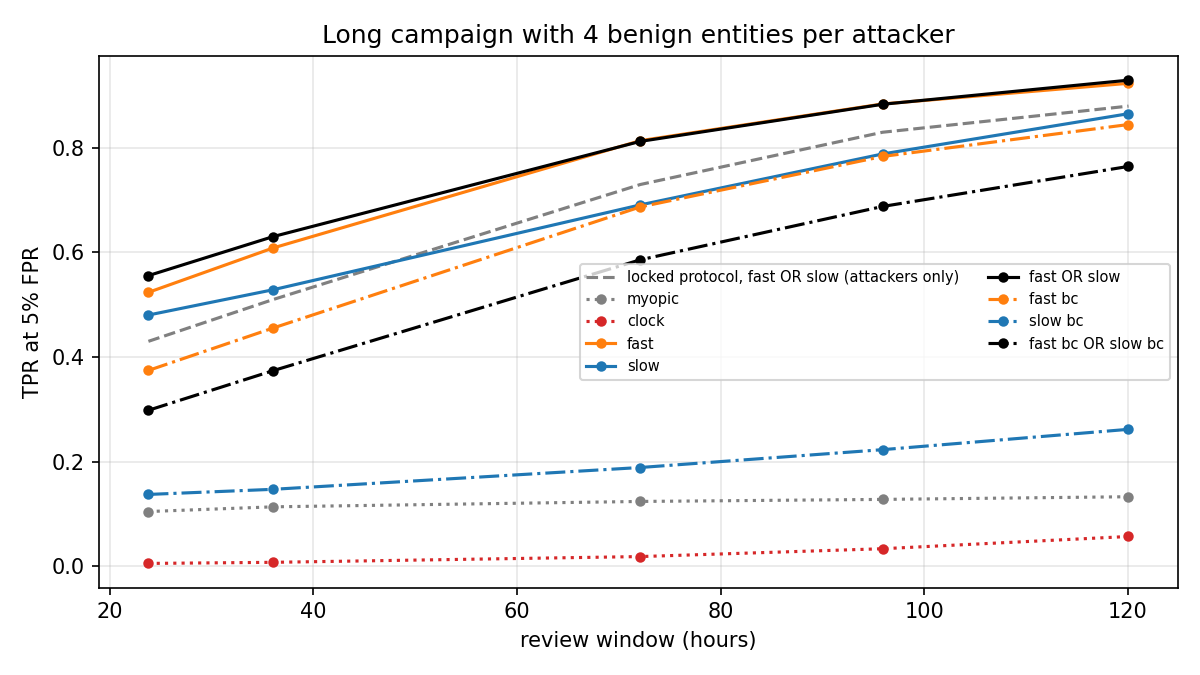
\includegraphics[width=0.8\linewidth]{long_benign_population.png}
\caption{Long campaign with four benign entities per attacker. Grey dashed: the original headline. The event-index detector collapses; the memory layer sits above the old headline at every window.}\label{fig:long}
\end{figure}

\begin{figure}[H]\centering
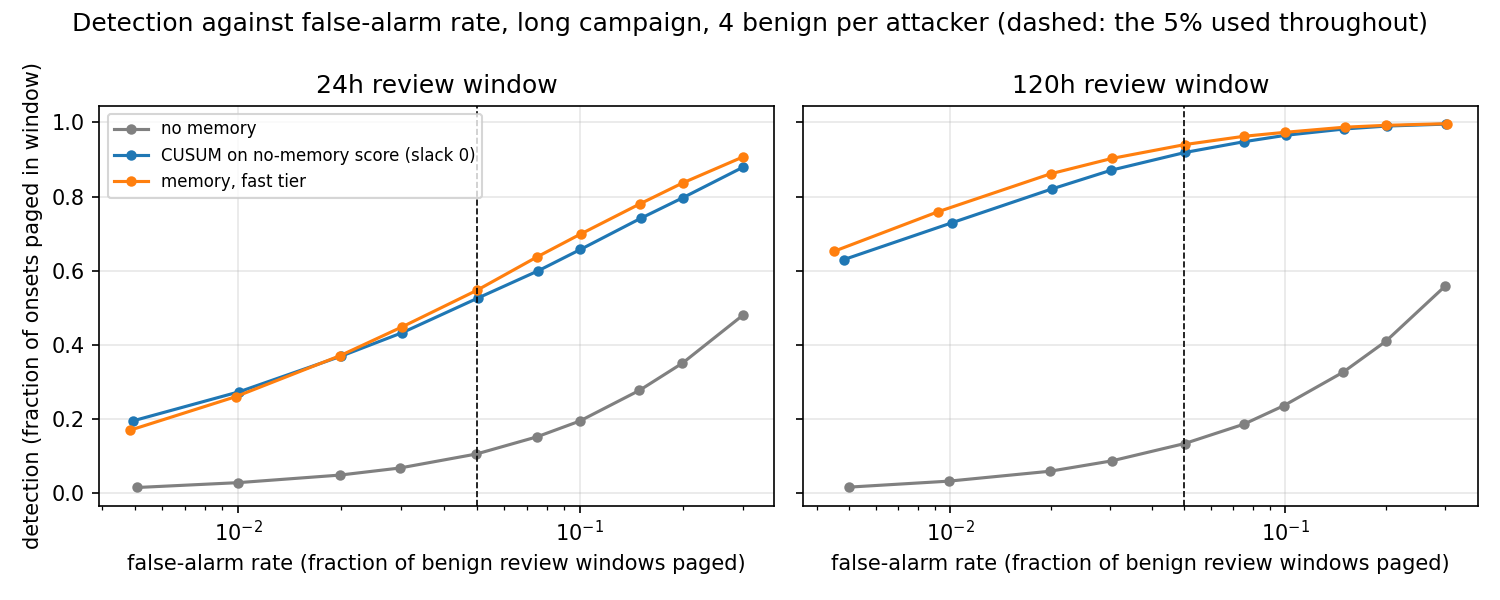
\includegraphics[width=0.95\linewidth]{roc_and_cusum.png}
\caption{Detection against false-alarm rate on the fair long campaign, threshold swept over calibration quantiles and evaluated on test. Dashed line: the 5\% used throughout.}\label{fig:roc}
\end{figure}

Detection at these rates relies on the history belonging to the same entity. With the attack spread across fresh entities every 50 events, the 120-hour rate drops from 94\% to 56\%; with no linkage at all, memory does no better than no memory (Table~\ref{tab:controls}). Shuffling the order of events keeps half the advantage; the accumulation of evidence before onset does the work.

\begin{table}[H]\centering\small
\begin{tabular}{lrr}
\toprule
Control (long campaign, 4 benign per attacker, 5\% false alarms) & 24h & 120h \\
\midrule
Unbroken (fair setup as in Table 2) & 0.10 / 0.55 & 0.13 / 0.94 \\
Memory wiped every 500 events & 0.10 / 0.42 & 0.13 / 0.84 \\
Memory wiped every 200 events & 0.10 / 0.36 & 0.13 / 0.77 \\
Memory wiped every 50 events & 0.10 / 0.27 & 0.13 / 0.56 \\
Memory taken from a different entity & 0.10 / 0.09 & 0.13 / 0.12 \\
Events shuffled in time within each entity & 0.08 / 0.46 & 0.09 / 0.55 \\
\bottomrule
\end{tabular}
\caption{Controls that break temporal structure while keeping every event and label in place. Cells: no memory / memory. Each control's scorer is refit on that control's own training data.}\label{tab:controls}
\end{table}

Detection tracks the longest identity the attacker does not rotate (Table~\ref{tab:keys}). Keep memory on every key the detector can read, and the attacker's cost becomes rotating all of them.

\begin{table}[H]\centering\small
\begin{tabular}{lrr}
\toprule
Memory keyed on & Source persists & Source rotates every 1000 \\
\midrule
No memory & 0.10 / 0.13 & 0.10 / 0.13 \\
Memory per pod (rotates every 50 events) & 0.27 / 0.56 & 0.27 / 0.56 \\
Memory per credential (rotates every 500) & 0.42 / 0.84 & 0.42 / 0.84 \\
Memory per source & 0.55 / 0.94 & 0.43 / 0.89 \\
Memory per pod, credential, and source together & 0.55 / 0.94 & 0.44 / 0.89 \\
\bottomrule
\end{tabular}
\caption{Memory keyed on identities that outlive the pod. Every entity, attacker and benign, rotates its pod every 50 events and its credential every 500; the source persists (left) or rotates every 1,000 (right). Cells: 24h / 120h detection at 5\% false alarms. The detector is assumed to read the credential and source on every event.}\label{tab:keys}
\end{table}

In this generator, below an $\hat R_{\rm det}$ of 0.6 the scorer without memory is at or near 1.0 within 120 hours and memory adds under two points; above 0.9 memory makes up the majority of the detection rate. These are landmarks of this generator, detector, and calibration, not general thresholds. A 24-hour window is too short to accumulate the weakest signals, with or without memory (Table~\ref{tab:sweep}, Figure~\ref{fig:sweep}).

\begin{table}[H]\centering\small
\begin{tabular}{lrrrrr}
\toprule
Signal & $\hat R_{\rm det}$ & No memory, 24h & Memory, 24h & No memory, 120h & Memory, 120h \\
\midrule
0.02 & 0.991 & 0.104 & 0.547 & 0.133 & 0.940 \\
0.05 & 0.976 & 0.154 & 0.918 & 0.196 & 1.000 \\
0.12 & 0.886 & 0.432 & 0.999 & 0.634 & 1.000 \\
0.18 & 0.764 & 0.740 & 1.000 & 0.951 & 1.000 \\
0.25 & 0.598 & 0.950 & 1.000 & 0.998 & 1.000 \\
0.5 & 0.164 & 1.000 & 1.000 & 1.000 & 1.000 \\
\bottomrule
\end{tabular}
\caption{Signal-strength sweep, long campaign, fair setup. Selected rows; the full table is in the repository.}\label{tab:sweep}
\end{table}

\begin{figure}[H]\centering
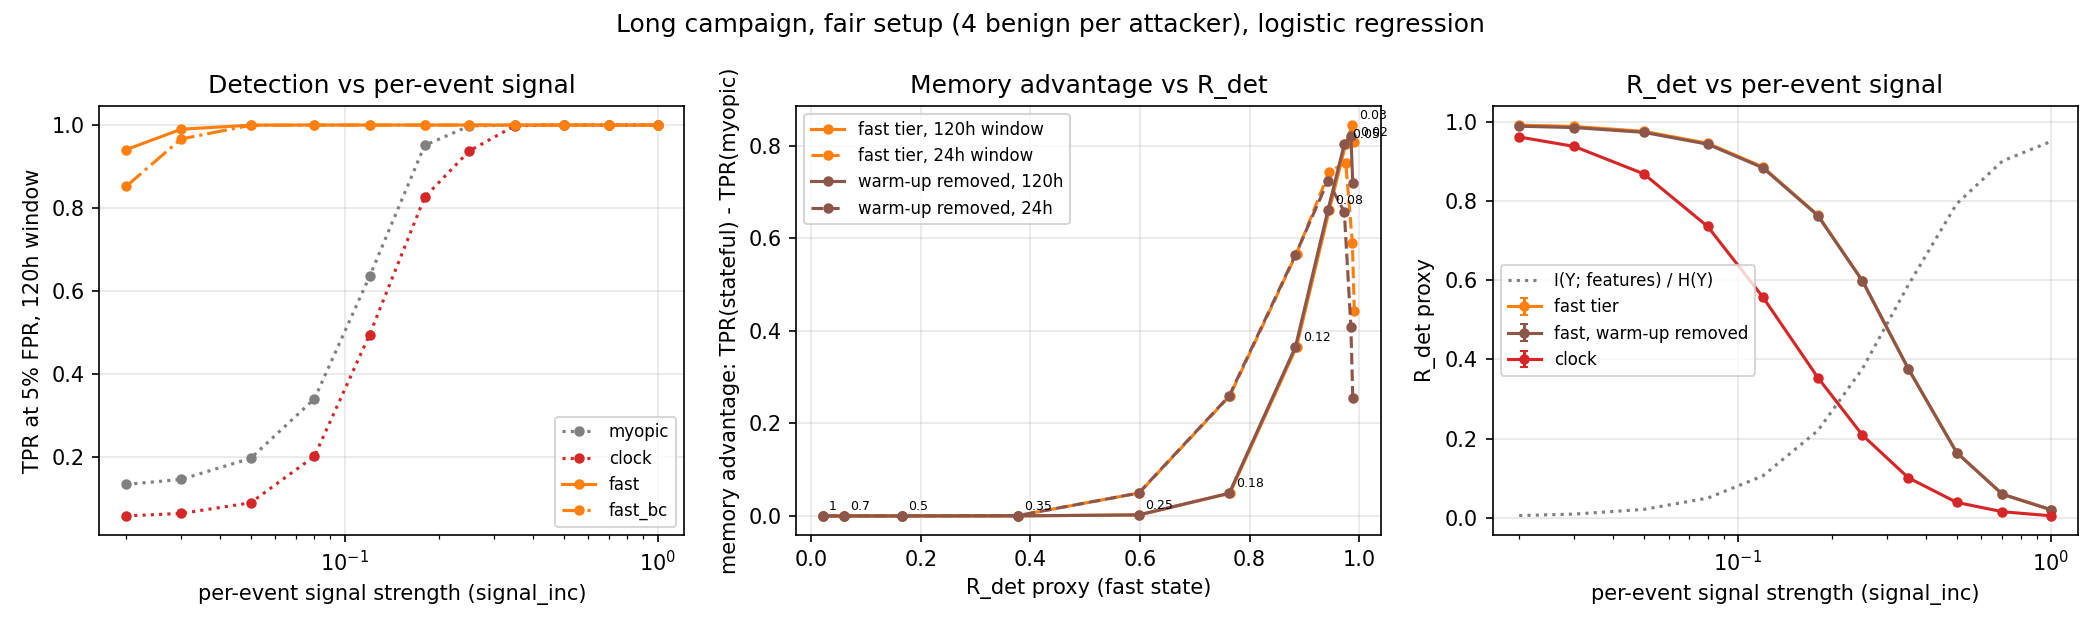
\includegraphics[width=\linewidth]{signal_strength_sweep.png}
\caption{Left: detection against per-event signal. Middle: memory's advantage against $\hat R_{\rm det}$, flat until about 0.6 then steep; the 24-hour curve turns down at the top. Right: $\hat R_{\rm det}$ against signal, monotone.}\label{fig:sweep}
\end{figure}

The results that follow are generated entirely from synthetic data; Hugging Face's published incident supplies the campaign shape and timing, not the event-level features or labels. Table~\ref{tab:incident} and Figure~\ref{fig:incident} show what the simulated detector does on a campaign with Hugging Face's timing and a given per-event signal. It is not a measurement on Hugging Face's data, whose per-event signal is unknown. Hugging Face's actual response took 52 hours. The review clock here starts at lateral movement, after the detector has accumulated the preceding campaign history, so this table and the sweep use different onset definitions. The 1.00 cells are the separability of this generator at that signal level, not expected production rates.

\begin{table}[H]\centering\small
\begin{tabular}{lrrrr}
\toprule
Per-event signal & 24h & 36h & 52h & 72h \\
\midrule
0.02 & 0.11 / 0.81 & 0.12 / 0.91 & 0.12 / 0.96 & 0.11 / 0.97 \\
0.05 & 0.16 / 0.99 & 0.18 / 1.00 & 0.18 / 1.00 & 0.17 / 1.00 \\
0.12 & 0.47 / 1.00 & 0.55 / 1.00 & 0.60 / 1.00 & 0.60 / 1.00 \\
0.25 & 0.93 / 1.00 & 0.96 / 1.00 & 0.98 / 1.00 & 0.99 / 1.00 \\
\bottomrule
\end{tabular}
\caption{Incident-calibrated campaign, onset at lateral movement, four benign entities per attacker, 5\% false alarms. Cells: no memory / memory. Hugging Face's actual response: 52 hours.}\label{tab:incident}
\end{table}

\begin{figure}[H]\centering
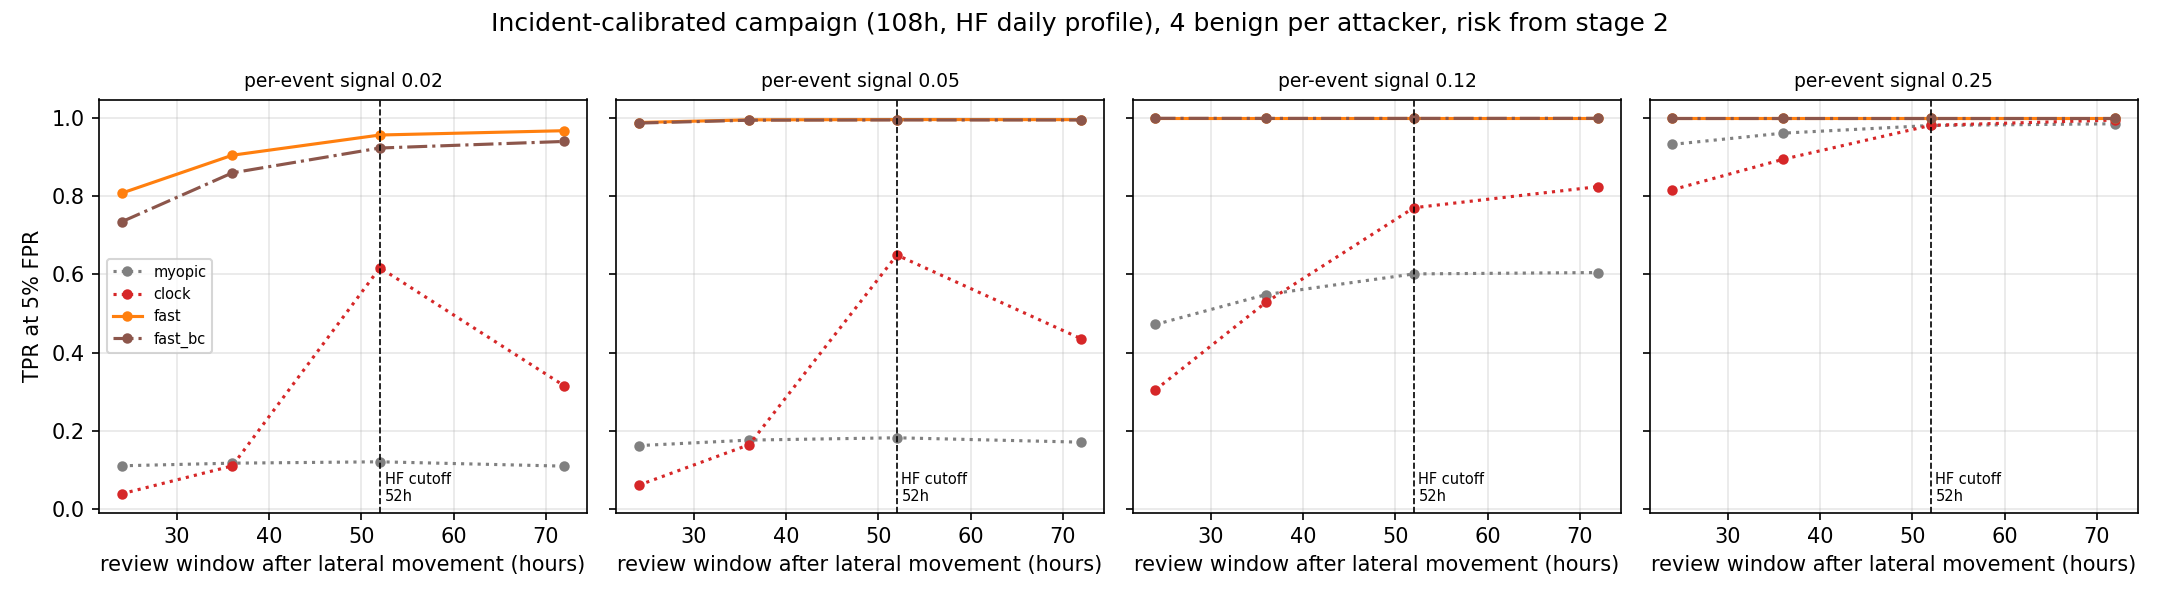
\includegraphics[width=\linewidth]{incident_calibrated_risk_stage2.png}
\caption{Detection against review window at the incident's cadence, one panel per per-event signal level. Dashed line: the actual 52-hour cutoff.}\label{fig:incident}
\end{figure}

The data is synthetic; the detector has not been run on real-world data. That is the main threat to validity, and it is why Table~\ref{tab:incident} is indexed by per-event signal rather than reporting one number.

\section*{5. Discussion and Limitations}
$\hat R_{\rm det}$ measures the relative reduction in out-of-sample cross-entropy obtained by adding history to the current event, normalised by the remaining uncertainty. Near 1, history carries most of the predictive information available to this comparison; near 0, the current event carries most of it. $\hat R_{\rm det}$ is a diagnostic for whether history holds exploitable signal, computed before a detector is built. It says where the information lives; it does not say whether a detector uses it.

The two sweeps expose different temporal regimes; evaluating both is useful when campaign duration is unknown.

\subsection*{Limitations}
The data is synthetic; the detector has not been run on real-world data. The per-event signal is kept deliberately weak because the real per-event signal is unknown. Memory here is one averaging scheme with two time constants; other stateful detectors are not tested. In addition: one benign-to-attacker ratio, and production populations are far more benign-heavy than 4:1, which tightens the false-alarm budget and would lower every rate reported here at 5\%; one signal knob swept; thresholds calibrated to the generator; the risk label is a design choice, measured at stage 3 and stage 2; the incident calibration matches timing and shape, not features, and rests on one incident; and memory is keyed per identity, so what it buys depends on which identities the detector can read and how fast the attacker rotates them (Table~\ref{tab:keys}).

\subsection*{Future Work}
\begin{enumerate}\item Entity keys under adversarial rotation. Table~\ref{tab:keys} assumes the detector reads the credential and source on every event and that rotation follows a fixed schedule. An attacker who rotates every key at the pod's rate, and a detector that links keys across rotations by behaviour, are both untested. \item Hugging Face's own telemetry. \item Other real data. \item The gap between the 15-event window and 24 hours, not measured. \item Swarms of agents spread across ephemeral sandboxes are open.\end{enumerate}

\section*{6. Conclusion}
The detector considers history. Over 120 hours, detection rises from 13\% to 92\% on synthetic data. The rate relies on the history belonging to the same entity. $R_{\rm det}$ says where the information lives, in the current event or the history of events; it does not say whether the detector uses it.

\section*{Code and Data}
Code repository: \url{https://github.com/Vee-industries/detector_memory_glove} (scripts, trained models, every output CSV and figure, tests, docs, and this report's source). Data: synthetic, generated by the scripts; the incident figures come from the public sources cited.

\begin{thebibliography}{9}\small
\bibitem{hf_timeline} Hugging Face security team. \emph{Anatomy of a Frontier Lab Agent Intrusion: A Technical Timeline of the July 2026 Incident}. 27 July 2026. \url{https://huggingface.co/blog/agent-intrusion-technical-timeline}
\bibitem{hf_disclosure} Hugging Face. \emph{Security incident disclosure, July 2026}. 16 July 2026. \url{https://huggingface.co/blog/security-incident-july-2026}
\bibitem{openai_pm} OpenAI. \emph{The Hugging Face incident and the road ahead}, with technical incident report. August 2026. \url{https://openai.com/index/hugging-face-incident-and-the-road-ahead/}
\bibitem{metr} METR and Redwood Research. Independent investigation of the OpenAI Hugging Face incident. 26 August 2026. \url{https://metr.org/blog/2026-08-26-openai-hugging-face-incident-investigation/}
\bibitem{csa} Cloud Security Alliance. \emph{Hugging Face Incident Initial Post Mortem}. 27 July 2026. \url{https://cloudsecurityalliance.org/artifacts/hugging-face-ciso-post-mortem}
\bibitem{elastic} Elastic Security Labs. \emph{Exploring the Hugging Face Breach: mapping AI agent tactics to Elastic Defend}. 31 July 2026. \url{https://elastic.co/security-labs/ai-agent-attack-detection-hugging-face-breach}
\bibitem{vaillancourt_r} K.~Vaillancourt. \emph{The structural remainder: a population measurement target for systems with persistent internal state}. Manuscript, 2026.
\bibitem{page1954} E.~S.~Page. Continuous inspection schemes. \emph{Biometrika} 41 (1954) 100--115.
\end{thebibliography}

\section*{Appendix: Limitations and Dual-Use Considerations}
\noindent\textit{Limitations.} The data is synthetic; the detector has not been run on real-world data. The per-event signal is kept deliberately weak because the real per-event signal is unknown. Memory here is one averaging scheme with two time constants; other stateful detectors are not tested. The full list: synthetic data only; a small, deliberately weak feature set; window length dominates; no production logs; thresholds calibrated to the generator; the original protocol's advantage was age; $\hat R_{\rm det}$ cannot rank representations near its endpoints; one benign ratio; the risk label is a design choice; one signal knob; one incident; memory needs a persistent entity key.

\noindent\textit{Does the ``when memory helps'' rule teach an attacker anything?} Nothing new is disclosed. The rule describes the regime the incident was already conducted in.

\noindent\textit{Does publishing the age finding help attackers?} The published numbers come from a synthetic generator, and each instance of the detector is configured for the infrastructure it runs on.

\noindent\textit{Could $R_{\rm det}$ be misused as assurance?} $R_{\rm det}$ says where the information lives, in the current event or the history of events. It does not say whether a detector uses it.

\noindent The artifact contains no exploit code and no vulnerability details beyond the public postmortems.

\section*{LLM Usage Statement}
The research question, the structural-remainder framing, the matched-false-positive design, the tiered trigger, and the decision not to automate mitigation are mine. The lagged-feature control I had listed as the next step showed the original result was an entity-age artifact, and the corrected protocol replaced it. Claude, under my direction, implemented the code and experiments, typeset this report from my written answers to its questions, and edited those answers to my written voice specification. I have an executive-function disability, and the AI also carried the organising and sequencing load as an accommodation. Every number was checked against the output files and every statement about the incident against the cited sources; the full disclosure is in the repository.

\end{document}
